\documentclass[12pt,leqno]{article}

\usepackage{indentfirst}

\usepackage{graphicx}
\graphicspath{ {./img/} }

\textwidth              16 cm
\textheight             23 cm
\oddsidemargin          -1 cm
\evensidemargin         -1 cm
\topmargin              -1 cm
\setlength{\evensidemargin}{15.5pt}
\setlength{\oddsidemargin}{2.5pt}

\pagestyle{empty}

\def\ClasaO{{\mathcal O}}

\usepackage{array}
\newcolumntype{P}[1]{>{\centering\arraybackslash}p{#1}}

\usepackage{multirow}
\usepackage{subcaption}
\usepackage{hyperref}

\usepackage{pgfplots}
\pgfplotsset{width=5in,compat=1.9}

\title{Finding global minimum using genetic algorithms}
\author{Stamate Valentin 2B4}

\begin{document}

\maketitle

\section*{Abstract}

  In this raport we will study the behaviour of a genetic algorithm solving a common optimization problem. Here will be explinations on how it works, the parameters, and based of the results concluzion.

\section{Introduction}
  The raport contain the interpretation of the results returned by a genetic algorithm solving a common problem. This way I made more sections for clarity:
  methods: there is the description of the algorithm used as well as how a candidate is reprezented, stop condition etc., description: contains details about the input size, precizion, repetions etc.
  results: tables with results and also few graphics to interpret the results, comparisons: a discution on how well the algorithm behaved, conclusion and a bibliografy: a list with all the sources I used for making the algorithm.
  

\subsection{Motivation}
  
  Genetic algorithms are inspired from nature and so far every species have evolved in such a way that they fit in the enviroment they are. So, making the same thing in code with a population we may expect a similar result with an enviroment set by us.
  The motivation is to see if such an algorithm give good results. If it does, this approach can be used in optimization problems that don't have a deterministic solution in polinomial time.

\section{Methods}
  
  The algorithm used is a genetic algorithm. The idea is to have a random population at the beginning that evolves over time. This way we can select a random number of candidates and multiply them two by two making two childrens that are added to population.
  For every generation the candidates are picked in such a way that the best of them have a higher chance of being selectd for the next generation keeping the population constant. The selection of the population is made with $ tourney \; selection $. 
  
  A member of population can be reprezented as a class with fields for assigning the radom selection and current fitness
  and the genome. The genome is reprezented as a bitstring that contains all the components for a point, because the mutations can be made very easy and we work with data. 

  The fitness for every candidate is calculated this way $ P(i).fit = 1 / ( - min(P) * cd + F(P(i).gene) + 100) $ where, $ cd $ is 1 if $ min(P) $ is negative, 0 otherwise $min(P)$ is the minimum value found within members, $P$ is the population and $F(gene)$ is the value of the function with the point as a bitstring. This way we keep a positive fitness even if the function takes negative numbers and we don't need to know the global minimum.
  
  We add $100$ to the formula to avoid having $1 / 0$ and to assing a fitness of $0.01$ for the best candidate when $cd$ is 1.
  
  The stop condition is when the number of generations reaches 1000.

  Finally, the mutation is made for every candidate and every genome component has a probability of 0.1\% to be changed. Without it, if we have a population with the same genome, it won't change.


\section{Experimental Setup}
  To have a better idea of how the algorithm is behaving we use different inputs and functions: as function dimention 2, 5, 10, 30 and functions: \href{http://www.geatbx.com/docu/fcnindex-01.html#P89_3085}{\textbf{DeJong's function}}, \href{http://www.geatbx.com/docu/fcnindex-01.html#P150_6749}{\textbf{Schwefel's function}},
  \href{http://www.geatbx.com/docu/fcnindex-01.html#P140_6155}{\textbf{Rastrigin's function}} and \href{http://www.geatbx.com/docu/fcnindex-01.html#P204_10395}{\textbf{Michalewicz's function}}. Each function have a different number of global minimums. The precision for the experiment is 5 so $ \varepsilon = 0.00001 $. The mutations probability is 0.1\% as explained earlier.
  The number of iterations is the same number as the stop condition witch is 1000 iterations/generations and the sample size is 30. The population size is 100 and the crossover probability is 20\%.

  CPU : Intel i5 - 8265U with 4 phisical and 8 virtual cores.

  Software: Visual Studio Code

  Programming Language: C++ 11

  The reprezentation of the functions have two dimensions and below evey image is the funtion definition, the interval and the global minimum.
  
  \begin{figure}[bp!]
    \centering
    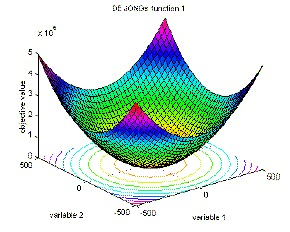
\includegraphics[width=0.4\linewidth, height=5cm]{dejong.jpg} 
    \caption*{De Jong's function: $ f_n(x) = \sum_{i=1}^{n} i x_i^2 $ $\; -5.12 \leq x_i \leq -5.12 $, $\; f(x) \geq 0 $}
  \end{figure}
  
\vfill

\begin{figure}[bp!]
  \centering
  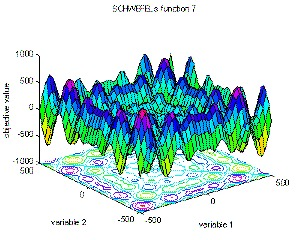
\includegraphics[width=0.4\linewidth, height=5cm]{schwefel.jpg}
  \caption*{Schwefel's function: $ f_n(x) = \sum_{i = 1}^{n}-x_i sin(\sqrt{|x_i|}) , -500 \leq x_i \leq 500 , f_n(x) \geq -n * 418.9829$}
\end{figure}
    
\newpage
\vfill

\begin{figure}[bp!]
  \centering
  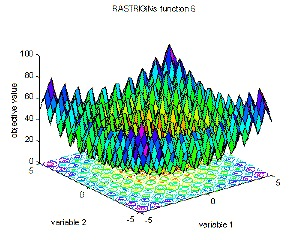
\includegraphics[width=0.4\linewidth, height=5cm]{rastrigin.jpg} 
  \caption*{Rastrigin's function: $ f_n(x) = 10n + \sum_{i = 1}^{n}(x_i^2 - 10 cos(2 \pi x_i)), -5.12 \leq x_i \leq 5.12, f(x) \geq 0 $}
\end{figure}
    
\begin{figure}[bp!]
  \centering
  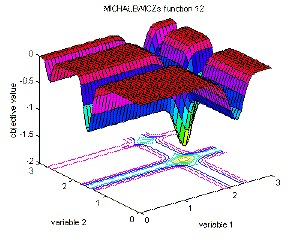
\includegraphics[width=0.4\linewidth, height=5cm]{michalenwicz.jpg}
  \caption*{Michalewicz's function: $ f_n(x) = -\sum_{i = 1}^{n} sin(x_i) (sin(i x_i^2 / \pi)) ^ 20, f_5(x) \geq -4.687, f_{10}(x) \geq -9.66$}  
\end{figure}

\vfill
\clearpage

\section{Results and Comparisons}

% 2
\begin{center}
  \begin{tabular}{|p{2.3cm}||p{3cm}|p{2cm}|p{2cm}|p{4.3cm}|} 
    \hline
    \multicolumn{5}{|c|}{2 dimensions} \\
    \hline
    Function    & Best Value & Mean & StDev & Duration \\ 
    \hline\hline
    De Jong     & $ 0.00496 $ & $ 0.50765 $ & $ 0.84868 $ & 7min 6s \\ 
    \hline
    Schwefel    & $ -837.96 $ & $ -815.6729 $ & $ 51.61495 $ & 9min 25s \\ 
    \hline
    Rastrigin   & $ 0.00067 $ & $ 2.70680 $ & $ 2.51859 $ & 7min 8s \\ 
    \hline
    Michalewicz & $ -0.80122 $ & $ -0.41647 $ & $ 0.33797 $ & 6min 51s \\ 
    \hline
 \end{tabular}
\end{center}

% 5
\begin{center}
  \begin{tabular}{|p{2.3cm}||p{3cm}|p{2cm}|p{2cm}|p{4.3cm}|} 
    \hline
    \multicolumn{5}{|c|}{5 dimensions} \\
    \hline
    Function    & Best Value & Mean & StDev & Duration \\ 
    \hline\hline
    De Jong     & $ 0.23029 $ & $ 1.48307 $ & $ 1.07994 $ & 18min 40s \\ 
    \hline
    Schwefel    & $ -2092.64 $ & $ -1932.087 $ & $ 113.9483 $ & 24min 14s \\ 
    \hline
    Rastrigin   & $ 0.81863 $ & $ 7.84385 $ & $ 3.28231 $ & 18min 46s \\ 
    \hline
    Michalewicz & $ -2.15064 $ & $ -1.38632 $ & $ 0.44637 $ & 18min 9s \\ 
    \hline
 \end{tabular}
\end{center}

% 10
\begin{center}
  \begin{tabular}{|p{2.3cm}||p{3cm}|p{2cm}|p{2cm}|p{4.3cm}|} 
    \hline
    \multicolumn{5}{|c|}{10 dimensions} \\
    \hline
    Function    & Best Value & Mean & StDev & Duration \\ 
    \hline\hline
    De Jong     & $ 1.20608 $ & $ 2.75918 $ & $ 1.14485 $ & 39min 42s \\ 
    \hline
    Schwefel    & $ -3993.25 $ & $ -3600.308 $ & $ 181.7103 $ & 51min 9s \\ 
    \hline
    Rastrigin   & $ 11.2655 $ & $ 18.72519 $ & $ 5.41844 $ & 39min 54s \\ 
    \hline
    Michalewicz & $ -4.48764 $ & $ -2.81137 $ & $ 0.80355 $ & 38min 36s \\ 
    \hline
 \end{tabular}
\end{center}

% 30
\begin{center}
  \begin{tabular}{|p{2.3cm}||p{3cm}|p{2cm}|p{2cm}|p{4.3cm}|} 
    \hline
    \multicolumn{5}{|c|}{30 dimensions} \\
    \hline
    Function    & Best Value & Mean & StDev & Duration \\ 
    \hline\hline
    De Jong     & $ 13.1106 $ & $ 20.1773 $ & $ 4.79230 $ & 1h 54min 41s \\ 
    \hline
    Schwefel    & $ -11169 $ & $ -10252.52 $ & $ 850.5401 $ & 1h 55min 19s \\ 
    \hline
    Rastrigin   & $ 74.966 $ & $ 132.1712 $ & $ 28.80329 $ & 1h 55min 22s \\ 
    \hline
    Michalewicz & $ -9.07803 $ & $ -7.16802 $ & $ 1.01378 $ & 1h 51min 36s \\ 
    \hline
 \end{tabular}
\end{center}

% plot
\begin{center}
  \resizebox*{9cm}{9cm}{
    \begin{tikzpicture}
      \begin{axis}[
          title={The input-time variation for Rastrigin's function},
          xlabel={Input [the number of components]},
          ylabel={Time [minutes]},
          xmin=0, xmax=30,
          ymin=0, ymax=120,
          xtick={0, 2, 5, 10, 30},
          ytick={0, 10, 30, 60, 120},
          legend pos=north west,
          ymajorgrids=true,
          grid style=dashed,
      ]
      
      \addplot[
          color=blue,
          mark=square,
          ]
          coordinates {
          (0, 0)(2, 7)(5, 18)(10, 39)(30, 115)
          };
          \addlegendentry{Function Evolution}
          
      \end{axis}
    \end{tikzpicture}
  }  
\end{center}
  
  We observe that the time increases linear with input witch is a good thing because it can be used in practice for bigger inputs also taking into consideration that the running time is low for such a problem.
  
\begin{center}
  \resizebox*{9cm}{9cm}{
    \begin{tikzpicture}
      \begin{axis}[
          title={Standard Deviation for Rastrigin's function},
          xlabel={Input [the number of components]},
          ylabel={Value},
          xmin=0, xmax=30,
          ymin=0, ymax=30,
          xtick={0, 2, 5, 10, 30},
          ytick={0, 10, 20, 30},
          legend pos=north west,
          ymajorgrids=true,
          grid style=dashed,
      ]
      
      \addplot[
          color=red,
          mark=square,
          ]
          coordinates {
          (2, 2.5)(5, 3.2)(10, 5.4)(30, 28.80)
          };
          \addlegendentry{Function Evolution}
          
      \end{axis}
    \end{tikzpicture}
  }
\end{center}

  The standard deviation looks like it's increasing exponentially but it's normal because once with the increase of input also the domain increases and we didn't increase the other parameters.

\newpage

Now, let's run the same algorithm but with mutation probability of 1\% and 0.01\% instead of 0.1\% to see what changes. 

\begin{center}
  \begin{tabular}{|p{2.3cm}||p{3cm}|p{2cm}|p{2cm}|} 
    \hline
    \multicolumn{4}{|c|}{Rastrigin's function with 30 dimensions} \\
    \hline
    Mut. Prob.    & Best Value & Mean & StDev \\ 
    \hline\hline
    $ 0.01\% $ & $ 111.938 $ & $ 174.0999 $ & $ 39.59821 $ \\ 
    \hline
    $ 0.1\%  $ & $ 74.966 $ & $ 132.1712 $ & $ 28.80329 $ \\ 
    \hline
    $ 1\%    $ & $ 297.874 $ & $ 335.4668 $ & $ 29.83531 $ \\ 
    \hline
 \end{tabular}
\end{center}

  We see that the result is the best when mutation probability is set to 0.1\%, better than when is set to 1\%. So making it smaller means better results?
  Not necessary. Decresing it down to 0.01\% there is almost no mutation and only crossover induce variation. This is why we get the worst result.


  Let's make another test but this time changing the probabilities one by one. The sample size is 10.
\begin{center}
  \begin{tabular}{|p{2.3cm}||p{3cm}|p{2cm}|p{2cm}|p{2cm}|} 
    \hline
    \multicolumn{5}{|c|}{Rastrigin's function with 10 dimensions} \\
    \hline
    Mut. Prob.  & Crossover & Best Value & Mean & StDev \\ 
    \hline\hline
    $ 0.1\%  $ & $ 20\% $ & $ 12.7081 $ & $ 17.00872 $ & $ 4.63378 $ \\ 
    \hline
    $ 0.1\%  $ & $ 100\% $  & $ 8.47128 $ & $ 16.63453 $ & $ 5.27540 $ \\ 
    \hline
    $ 75\%   $ & $ 20\% $ & $ 91.6142 $ & $ 110.7948 $ & $ 11.07916 $ \\ 
    \hline
 \end{tabular}
\end{center}

  The first row is from my normal results picking only 10 elements from sample. So, making the crossover 100\% we see that we get a better result. The crossover is made within all the population, meaning that there will be more candidates to choose and the next generation will contain more good candidates.
  Looking at the third row with mutation probability of 75\% the population suffers may mutation and if this probabilty would be increased to 100\% we willl obtain an algoritm similar to $ random \; search $. This is why we get the worst results here.


\section{Conclusions}
  We study a genetic algorithm solving the minimum of a function problem. The results are very good for such an alogrithm even if it doesn't give the best results for big inputs, they are still relevant.
  The time is pretty low and increases linear, so we can approximate how much it's gonna take for greater inputs. As a conclusion, genetic algorithms can be use in practice for solving many optimization problems because even if they don't give the best result at a certain time
  they give a very good approximation of it. 

\newpage

\begin{thebibliography}{9}
  \bibitem{}
    \url{https://stackoverflow.com/questions/39102028/how-to-return-vector-of-pointers-and-ownership-c11}
  \bibitem{}
    \url{https://stackoverflow.com/questions/11134497/constant-sized-vector}
  \bibitem{}
    \url{https://stackoverflow.com/questions/1380463/sorting-a-vector-of-custom-objects}  
  \bibitem{}
    \url{https://profs.info.uaic.ro/~eugennc/teaching/ga/}  
  \bibitem{}
    \url{https://www.youtube.com/watch?v=9zfeTw-uFCw&list=PLRqwX-V7Uu6bJM3VgzjNV5YxVxUwzALHV&ab_channel=TheCodingTrain}  
  \bibitem{}
    Seminar 5 notes
  \bibitem{}
    \url{http://www.geatbx.com/docu/fcnindex-01.html#P89_3085}
  \bibitem{}
    \url{http://www.geatbx.com/docu/fcnindex-01.html#P150_6749}
  \bibitem{}
    \url{http://www.geatbx.com/docu/fcnindex-01.html#P140_6155}
  \bibitem{}
    \url{http://www.geatbx.com/docu/fcnindex-01.html#P204_10395}

  \end{thebibliography}  
  


\end{document}